%!TEX root = ../main.tex

\section{Nominal fit}
\label{sec:bd2jpsiks:nominalfit}

A multi-dimensional fit to the distributions of the reconstructed mass $m$,
the decay time $t$ and its error prediction $\sigma_t$, the OS and SS\pion
tags and mistag probabilities is performed, mainly to extract the \CP
observables \SJpsiKS and \CJpsiKS. Thanks to the selection, which cleans up
the sample from other background contributions, besides the signal component
only the combinatorial background component needs to be parametrised.

The mass distribution, which enables the best discrimination of the two
components, is modelled by a modified Hypatia PDF~\cite{Santos:2013ky} and an
exponential function. All parameters are allowed to differ between the two
track type categories. The four tail parameters of the signal parametrisation
are taken from fits to simulated events.

The PDF describing the signal decay time distribution is basically given by
\begin{equation}
\begin{aligned}
  \frac{\mathrm{d}\Gamma(t,d)}{\mathrm{d}t}
  &\propto \mathrm{e}^{-t/\tau}
    \Big(
      1
      - d\, \Sf \sin{\left(\dm\,t\right)}
      + d\, \Cf \cos{\left(\dm\,t\right)}
    \Big)\,,
\end{aligned}
\label{eq:simpledecayrates}
\end{equation}
with $d = \num{+1}$ for \Bd and $d = \num{-1}$ for \Bdb. The decay width
difference \DGd is set to zero. The theoretical parametrisation is extended by
taking into account the production asymmetry and the experimental effects of
mistagging. Furthermore, it is convolved with the decay time resolution model
presented in \cref{sec:bd2jpsiks:decaytime:resolution} and multiplied by the
time-dependent efficiency correction for low and high decay times developed in
\cref{sec:bd2jpsiks:decaytime:acceptance}. The background decay time
distribution is parametrised with the sum of exponential functions. How many
of those give the best description in the various categories, in which the
whole data sample can be divided into, is determined in extensive studies
using sweighted background distributions (see
\cref{sec:bd2jpsiks:backgrounds}).

Lognormal distributions have been found to fit best when describing the decay
time error distributions. A combination of double and single lognormals with
some parameters being shared among the categories is used. Especially the
downstream and the long track distributions differ as can be seen in
\cref{fig:bd2jpsiks:nominalfit:time_error}.

\begin{figure}[htb]
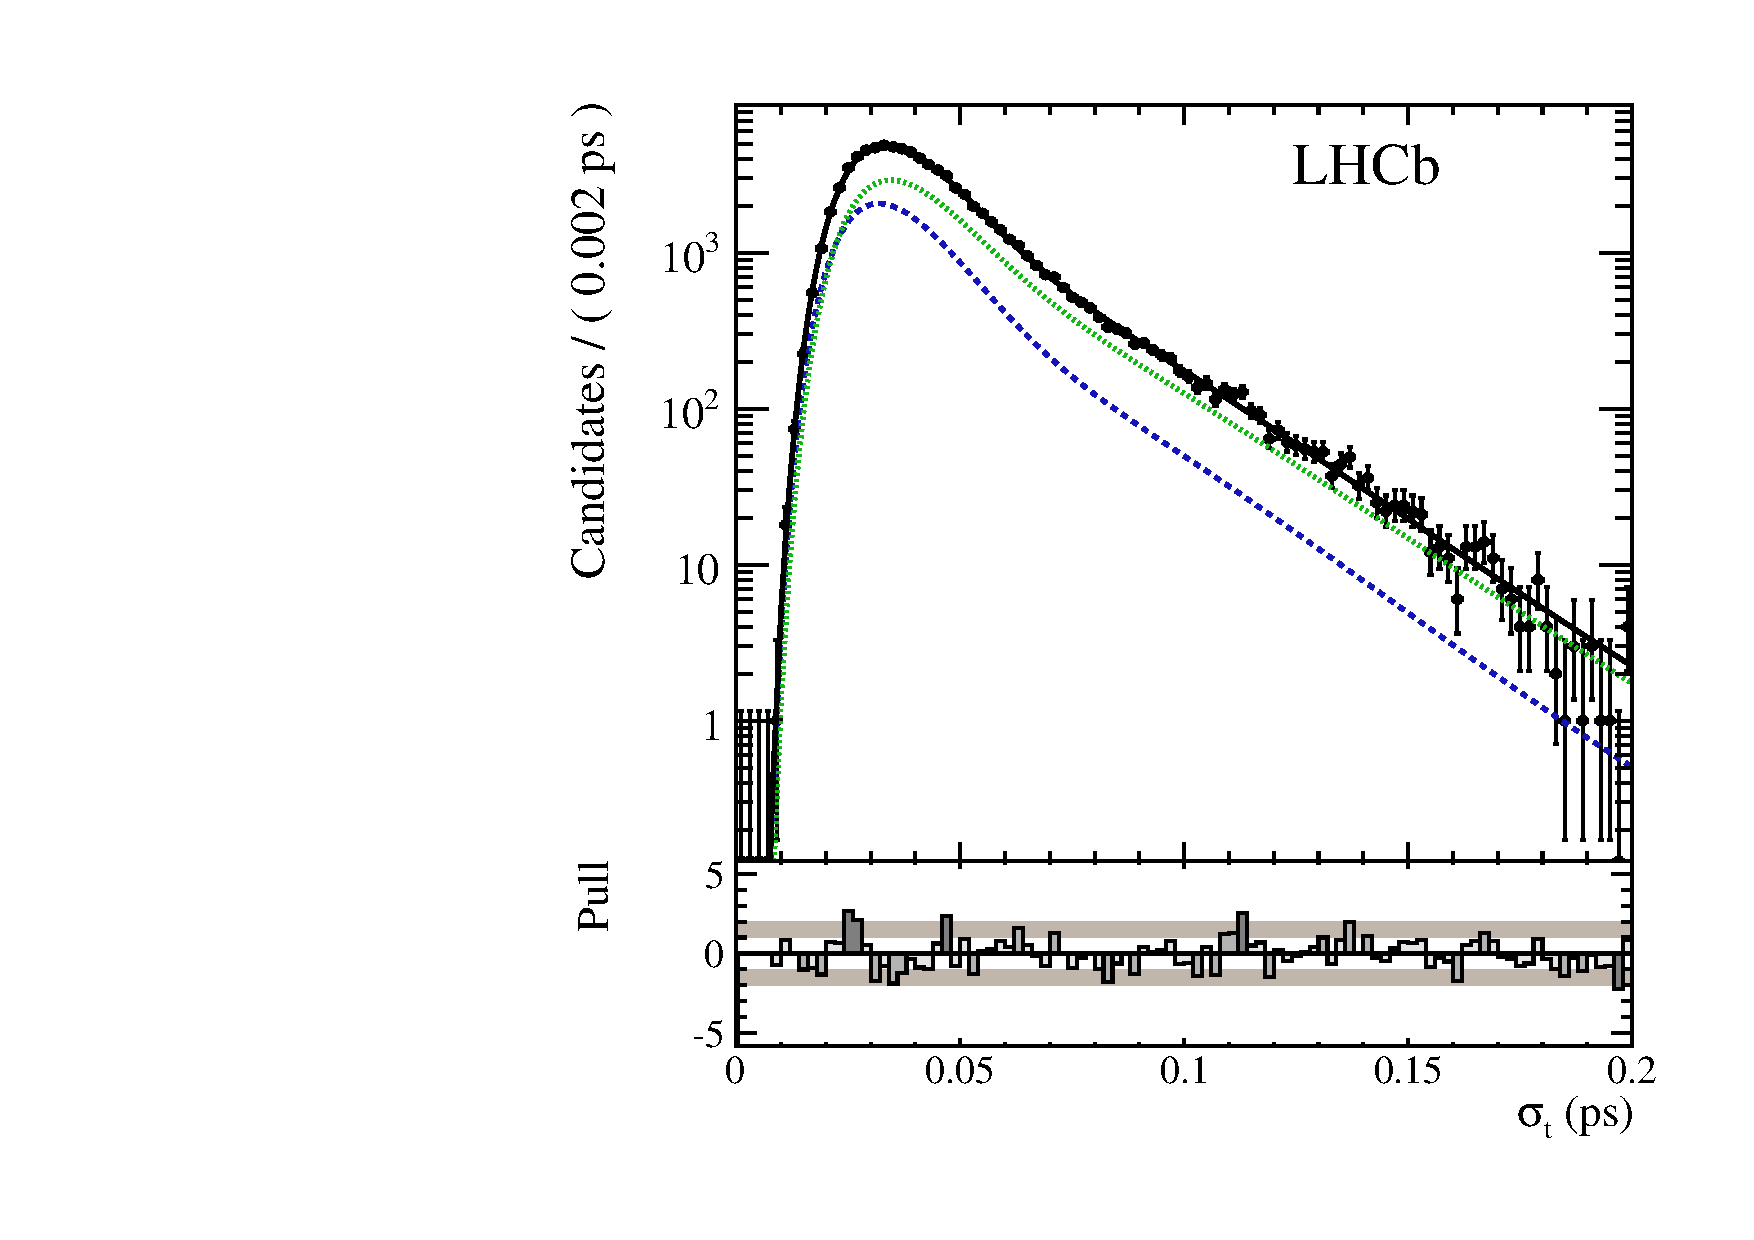
\includegraphics[width=0.49\textwidth]{06-Bd2JpsiKS/figs/obsTimeError_summed_pull_log_DD.pdf}
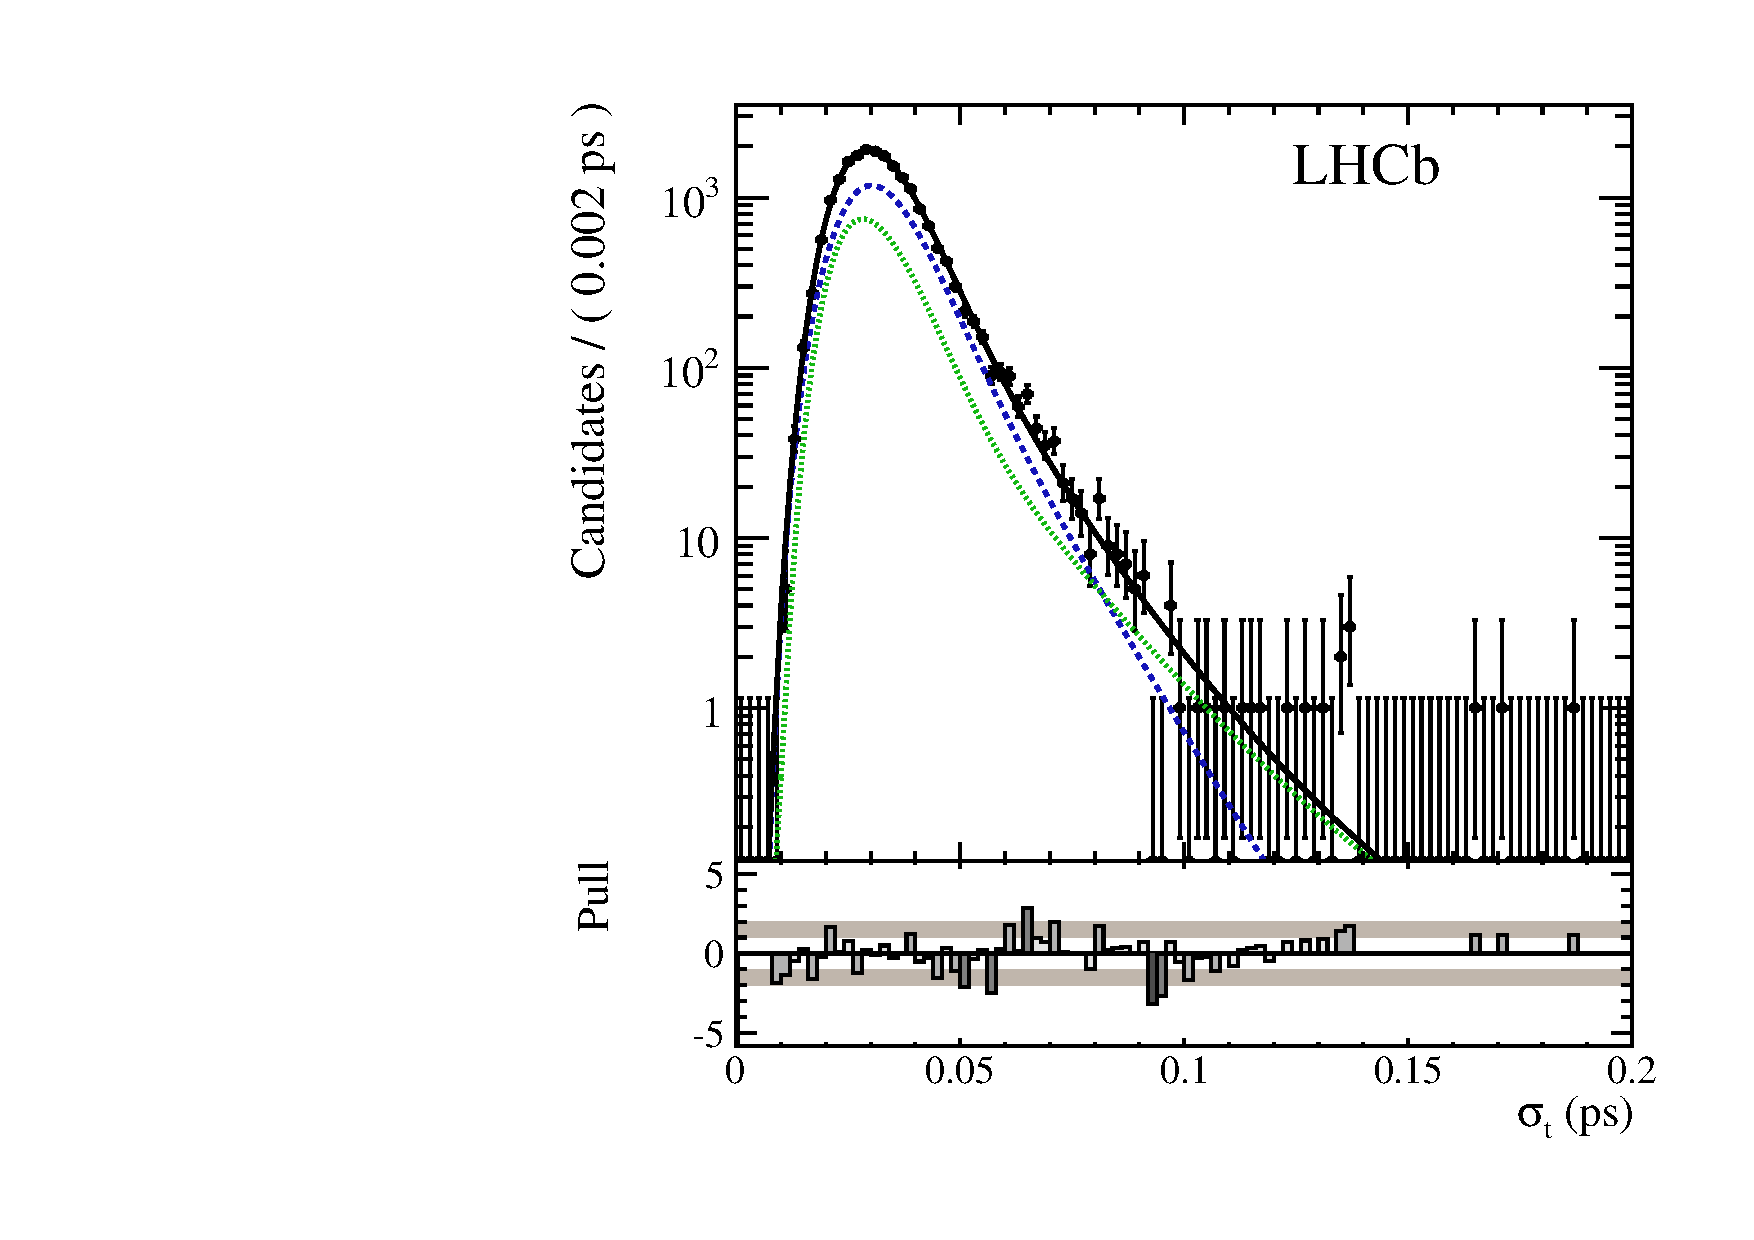
\includegraphics[width=0.49\textwidth]{06-Bd2JpsiKS/figs/obsTimeError_summed_pull_log_LL.pdf}
\caption{
Time error distributions of downstream (left) and long track (right). The solid black line
shows the fit projection, while the blue dashed (green dotted) line shows the
signal (background) component.}
\label{fig:bd2jpsiks:nominalfit:time_error}
\end{figure}
\todo{tikz version of time error plots}

The mistag distributions are described with cubic splines. The seven knots for
the SS\pion distribution, and similarly the 12 knots for the OS distribution,
are positioned where the shape visibly changes. It is checked that the two
mistag estimates are uncorrelated with each other and with the decay time, at
least within the available statistical precision. This allows to simply
multiply the corresponding PDFs.

In the fit 11 external input parameters are constrained within their
statistical uncertainties. These are the production asymmetries for
\SIlist{7;8}{\TeV}, for which the procedure is explained in more detail in
\cref{sec:b02dd:decaytimefit:constraints}, the oscillation frequency
\dmd~\cite{PDG2014} and the flavour-tagging calibration parameters
(\cref{sec:dataanalysis:taggingcalibration:jpsixcalibration}).

To stabilize the fit the decay time resolution parameters, the spline
coefficients of the mistag parametrisation, the decay time error parameters
and all parameters included in the decay time acceptance model are fixed.
Thus, \num{72} floating parameters remain for the fit, of which \num{48} are
yields.

From the \num{41560} flavour-tagged \BdToJPsiKS decays the \CP observables are determined to be
\begin{align*}
  \SJpsiKS &=  \phantom{-}0.731 \, \pm 0.035 \, \text{(stat)} \pm 0.020 \, \text{(syst)}\,, \\
  \CJpsiKS &=  			- 0.038 \, \pm 0.032 \, \text{(stat)} \pm 0.005 \, \text{(syst)}\,,
\end{align*}
with a statistical correlation of \num{0.483}. In these results corrections of
\num{+0.002} for \SJpsiKS and \num{-0.005} for \CJpsiKS are included, which
account for \CP violation in $\Kz$--$\Kzb$ mixing and different nuclear
cross-sections in material between \Kz and
\Kzb~\cite{Fetscher:1996fa,*Ko:2010mk}.

The distributions of the invariant mass and the decay time are depicted in
\cref{fig:bd2jpsiks:nominalfit:mass_and_time}.

\begin{figure}[htb]
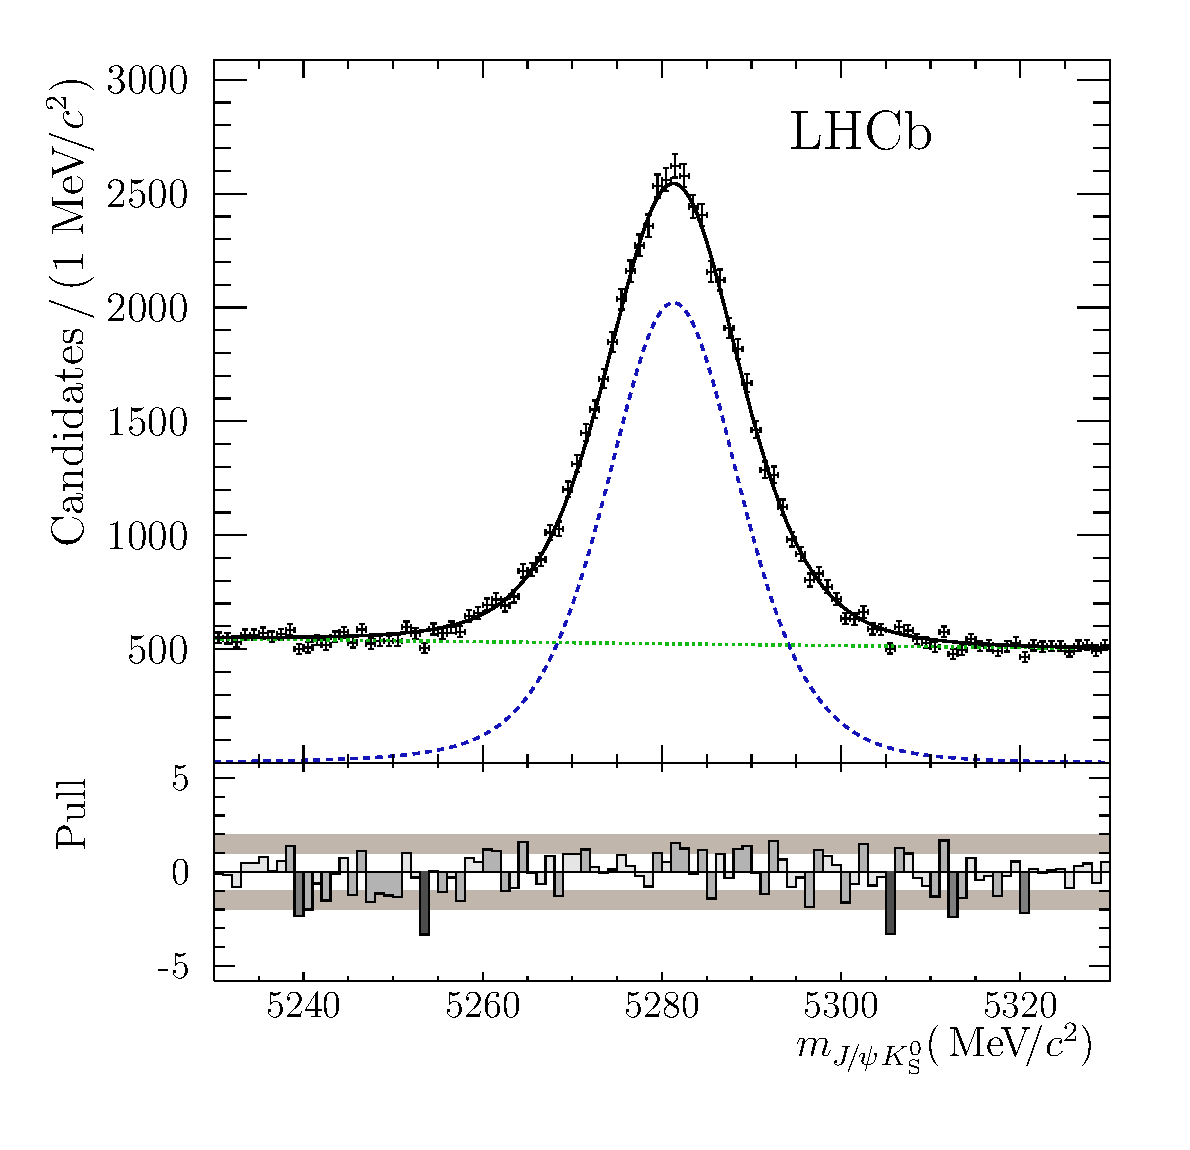
\includegraphics[width=0.49\textwidth]{06-Bd2JpsiKS/tikz/pdf/MassPulls_summed.pdf}
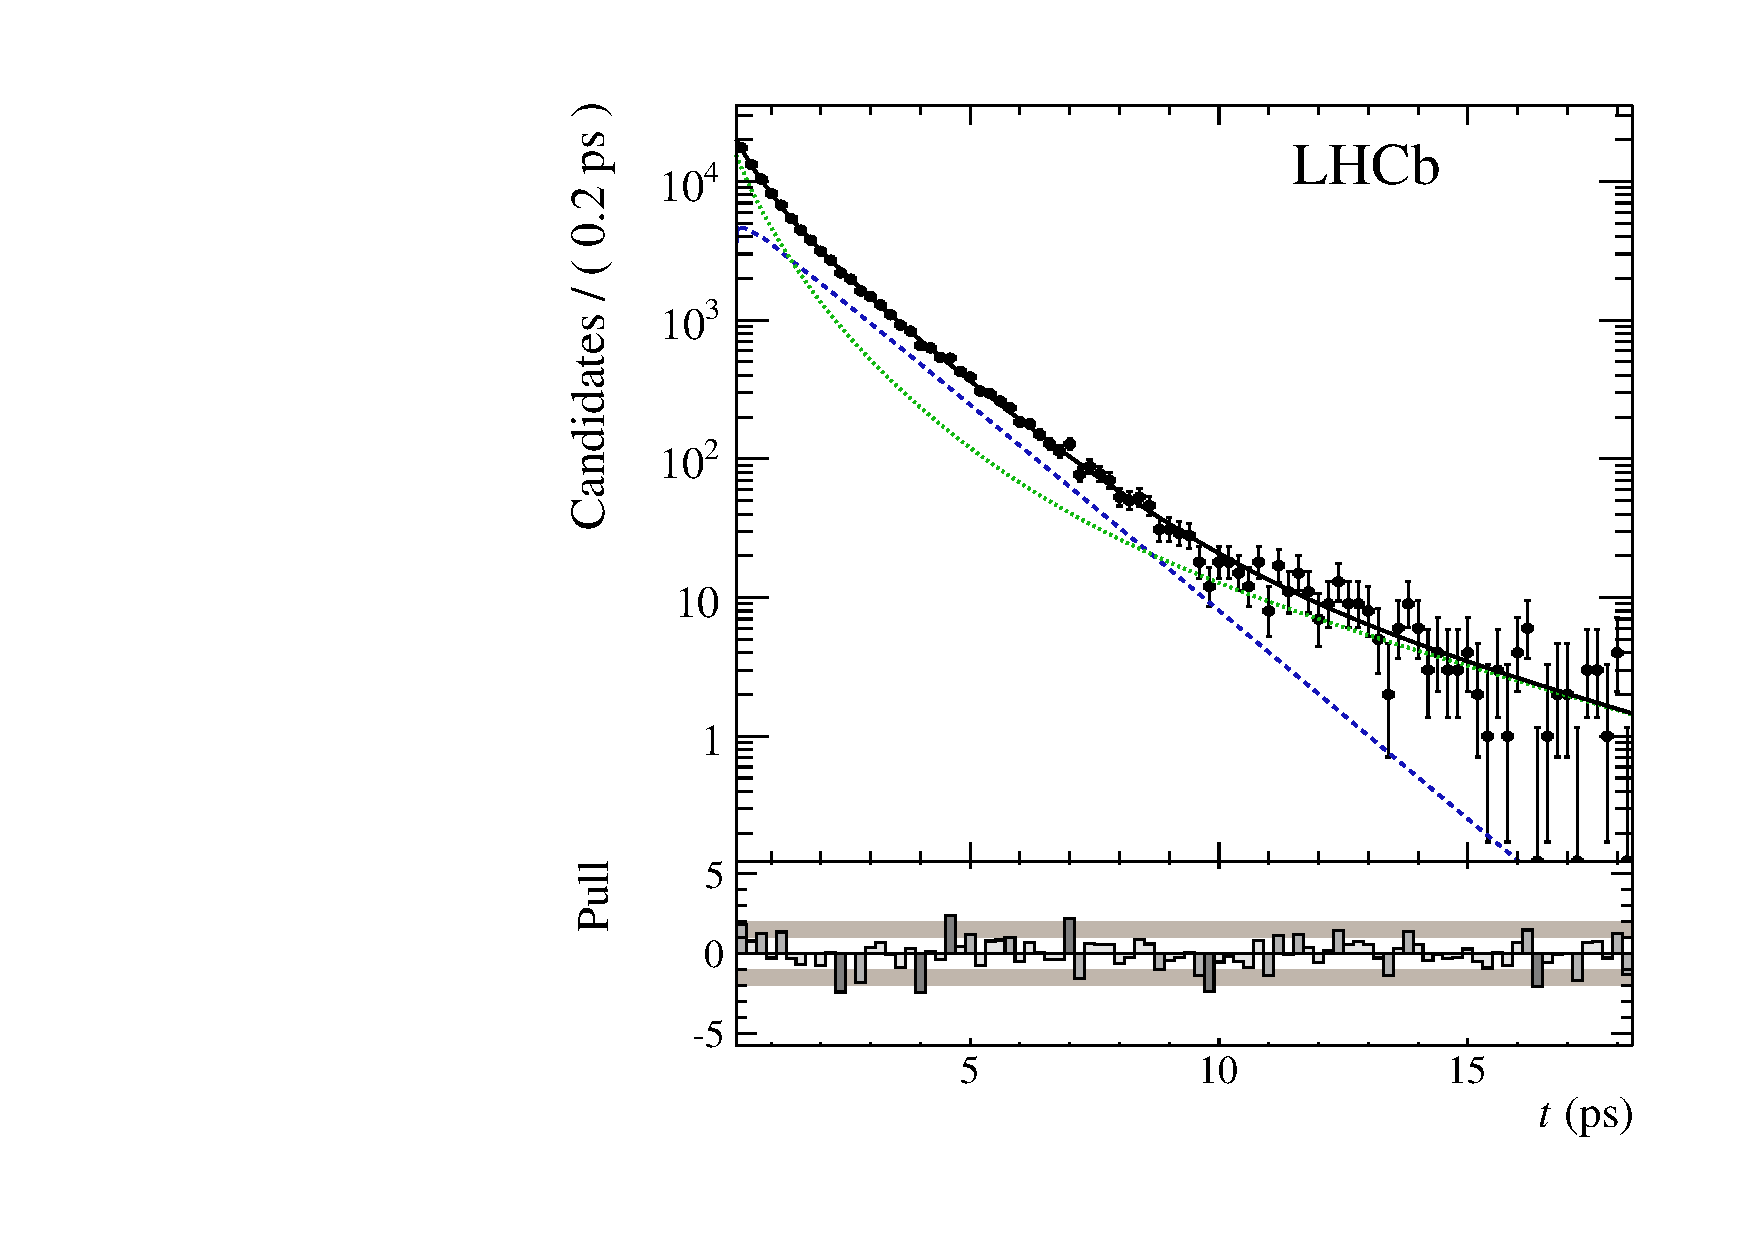
\includegraphics[width=0.49\textwidth]{06-Bd2JpsiKS/figs/obsTime_summed_pull_log.pdf}
\caption{
Invariant mass distribution (left) and decay time distribution (right). The solid black line
shows the fit projection, while the blue dashed (green dotted) line shows the
signal (background) component.}
\label{fig:bd2jpsiks:nominalfit:mass_and_time}
\end{figure}
\todo{decay time plot via tikz}